\begin{table}
\centering
\caption{Time taken to synchronize (in seconds) for 16 nodes in TOSSIM with different grid topologies, and different values of firing function constants (FFC). The - indicates cases in which synchronization is not achieved.} 
\label{tab:topologyFFC}
%%\subfigure[Table 1: Number of element]
\vspace{2pt}
\begin{tabular}{|r|r|r|r|r|} \hline
Topology                & {\bf FFC=10}  & {\bf FFC=50} & {\bf FFC=100} &   {\bf FFC=200}  \\ \hline
{\bf Grid}              &   90.70    &   73.55     &   84.24        &   266.89      \\ 
{\bf Ring}              &   -        &  123.55     &   77.87        &   194.83      \\ 
{\bf All-To-All}        &   98.43    &   23.44     &   59.35        &   227.05      \\ 
{\bf Line}              &   83.97    &   183.94    &   219.42       &   456.62      \\ \hline
\end{tabular}
\end{table}
\begin{table}
\centering
\caption{Average and Standard Deviation Statistics Per Topology for Table~\ref{tab:topologyFFC}.}
\label{tab:topologyStat}
%%\subfigure[Table 1: Number of element]
\vspace{2pt}
\begin{tabular}{|r|r|r|r|r|} \hline
Topology                & Average    & Standard Deviation \\ \hline
{\bf Grid}              & 128.85     & 92.30 \\ \hline  
{\bf Ring}              & 135.42     & 58.50  \\ \hline  
{\bf All-To-All}        & 102.07     & 88.77  \\ \hline  
{\bf Line}              & 235.99     & 157.87 \\ \hline  
\end{tabular}
\end{table}

\begin{figure}
\begin{center}
\includegraphics[width=1.1\hsize]{./figures/topFFC.pdf}
\end{center}
\caption{{\small {\bf The impact of topology and the magnitude of the firing function constant on the time to synchronize.
The exact values of the time taken to synchronize are listed in~\ref{tab:topologyFFC}.}}} 
\label{fig:topFFC}
\end{figure}

\begin{figure}[t]
\begin{center}
\includegraphics[width=1.0\hsize]{./figures/5-Jan-2005-1-RING-NODES-16-50CONSTANT-GROUP-PERIOD.pdf}
\end{center}
\caption{{\small {\bf Group period for 16 node ring topology with firing function constant 50.}}} 
%{\em This figure shows...}}}
\label{fig:rgp}
\end{figure}

\begin{figure}[t]
\begin{center}
\includegraphics[width=1.0\hsize]{./figures/5-Jan-2005-1-RING-NODES-16-50CONSTANT-GROUP-SPREAD.pdf}
\end{center}
\caption{{\small {\bf Group spread for 16 node ring topology with firing function constant 50.}}}
%{\em This figure shows...}}}
\label{fig:rgs}
\end{figure}

\begin{figure}[t]
\begin{center}
\includegraphics[width=1.0\hsize]{./figures/5-Jan-2005-1-LINE-NODES-16-50CONSTANT-GROUP-PERIOD.pdf}
\end{center}
\caption{{\small {\bf Group period for 16 node line topology with firing function constant 50.} }}
%{\em This figure shows...}}}
\label{fig:lgp}
\end{figure}

\begin{figure}[t]
\begin{center}
\includegraphics[width=1.0\hsize]{./figures/5-Jan-2005-1-LINE-NODES-16-50CONSTANT-GROUP-SPREAD.pdf}
\end{center}
\caption{{\small {\bf Group spread for 16 node line topology with firing function constant 50.} }}
%{\em This figure shows...}}}
\label{fig:lgs}
\end{figure}

\begin{figure}[t]
\begin{center}
\includegraphics[width=1.0\hsize]{./figures/5-Jan-2005-1-GRID-NODES-16-50CONSTANT-GROUP-PERIOD.pdf}
\end{center}
\caption{{\small {\bf Group period for 16 node 4by4 regular grid topology with firing function constant 50.} }}
%{\em This figure shows...}}}
\label{fig:ggp}
\end{figure}


\begin{figure}[t]
\begin{center}
\includegraphics[width=1.0\hsize]{./figures/5-Jan-2005-1-GRID-NODES-16-50CONSTANT-GROUP-SPREAD.pdf}
\end{center}
\caption{{\small {\bf Group spread for 16 node 4by4 regular grid topology with firing function constant 50.} }}
%{\em This figure shows...}}}
\label{fig:ggs}
\end{figure}


\begin{figure}[t]
\begin{center}
\includegraphics[width=1.0\hsize]{./figures/5-Jan-2005-1-ALL-NODES-16-50CONSTANT-GROUP-PERIOD.pdf}
\end{center}
\caption{{\small {\bf Group period for 16 node all-to-all topology with firing function constant 50.} }}
%{\em This figure shows...}}}
\label{fig:agp}
\end{figure}

\begin{figure}[t]
\begin{center}
\includegraphics[width=1.0\hsize]{./figures/5-Jan-2005-1-ALL-NODES-16-50CONSTANT-GROUP-SPREAD.pdf}
\end{center}
\caption{{\small {\bf Group spread for 16 node all-to-all topology with firing function constant 50.} }}
%{\em This figure shows...}}}
\label{fig:ags}
\end{figure}




\subsection{TOSSIM Experiments}
A number of simulation experiments have been performed on TOSSIM to evaluate
the impact of different parameters of the model on the accuracy and
quality of synchronicity achieved amongst the nodes.  We explore the impact
of parameters such as the firing function constant (a constant value that
is equal to $\frac{1}{\epsilon}$, where $\epsilon$ is the firing function
related quantity discussed in sections~\ref{sec:fireflyModel} and ~\ref{sec:firingFunc}), 
and the number of nodes on the quality of synchronicity achieved as 
measured by group spread, group period and time taken to synchronize.

Fig.~\ref{fig:topFFC} shows the values of time to synchronize for 16 nodes with different
topologies and firing function constants.  It is obvious that a higher firing function
constant does not imply consistently lower time to synchronization.  Overall nodes in the
line topology takes the longest time to synchronize except when the firing function constant
is 10. 
Nodes in the all-to-all topology generally take less time to synchronize than the other
topologies. This is not surprising since all-to-all is the best conceivable topology.
Tables~\ref{tab:topologyFFC}-~\ref{tab:topologyStat} show numerical values of the
time taken to synchronize (in seconds) for different topologies and firing function
constant values. The standard deviations give an idea of the large extent to
which the firing function constant can influence the time taken to achieve synchronicity.
In Table~\ref{tab:topologyStat} the line topology has the highest standard deviation,
and indicates that this topology is particularly vulnerable to changes in the firing function
constant.

Fig.~\ref{fig:rgp}-~\ref{fig:ags} show the group period and group spread of 16 nodes
with four different topologies: line, 4by4 regular grid, ring and all-to-all.
It is reassuring to see that for all node topologies, the group period stabalizes
at 1 after a given time period.  The group period of the line topology takes the
longest time to stabalize (190 seconds), while the group period of the all-to-all topology 
takes the shortest amount of time to stabalize (less than 30 seconds). Similarly
the group spread of the all-to-all topology has the least amount of variation,
and the group spread of the line topology has the most amount of variation.
The reason for this is quite intuitive. In the line topology, nodes towards the ends
of the lines have difficulty detecting all the fires. On the other hand, nodes in the
all-to-all connected topology are well connected to all their neighbors and
can efficiently respond to detected fires.


%% Geoff's graphs here

\begin{figure}[t]
\begin{center}
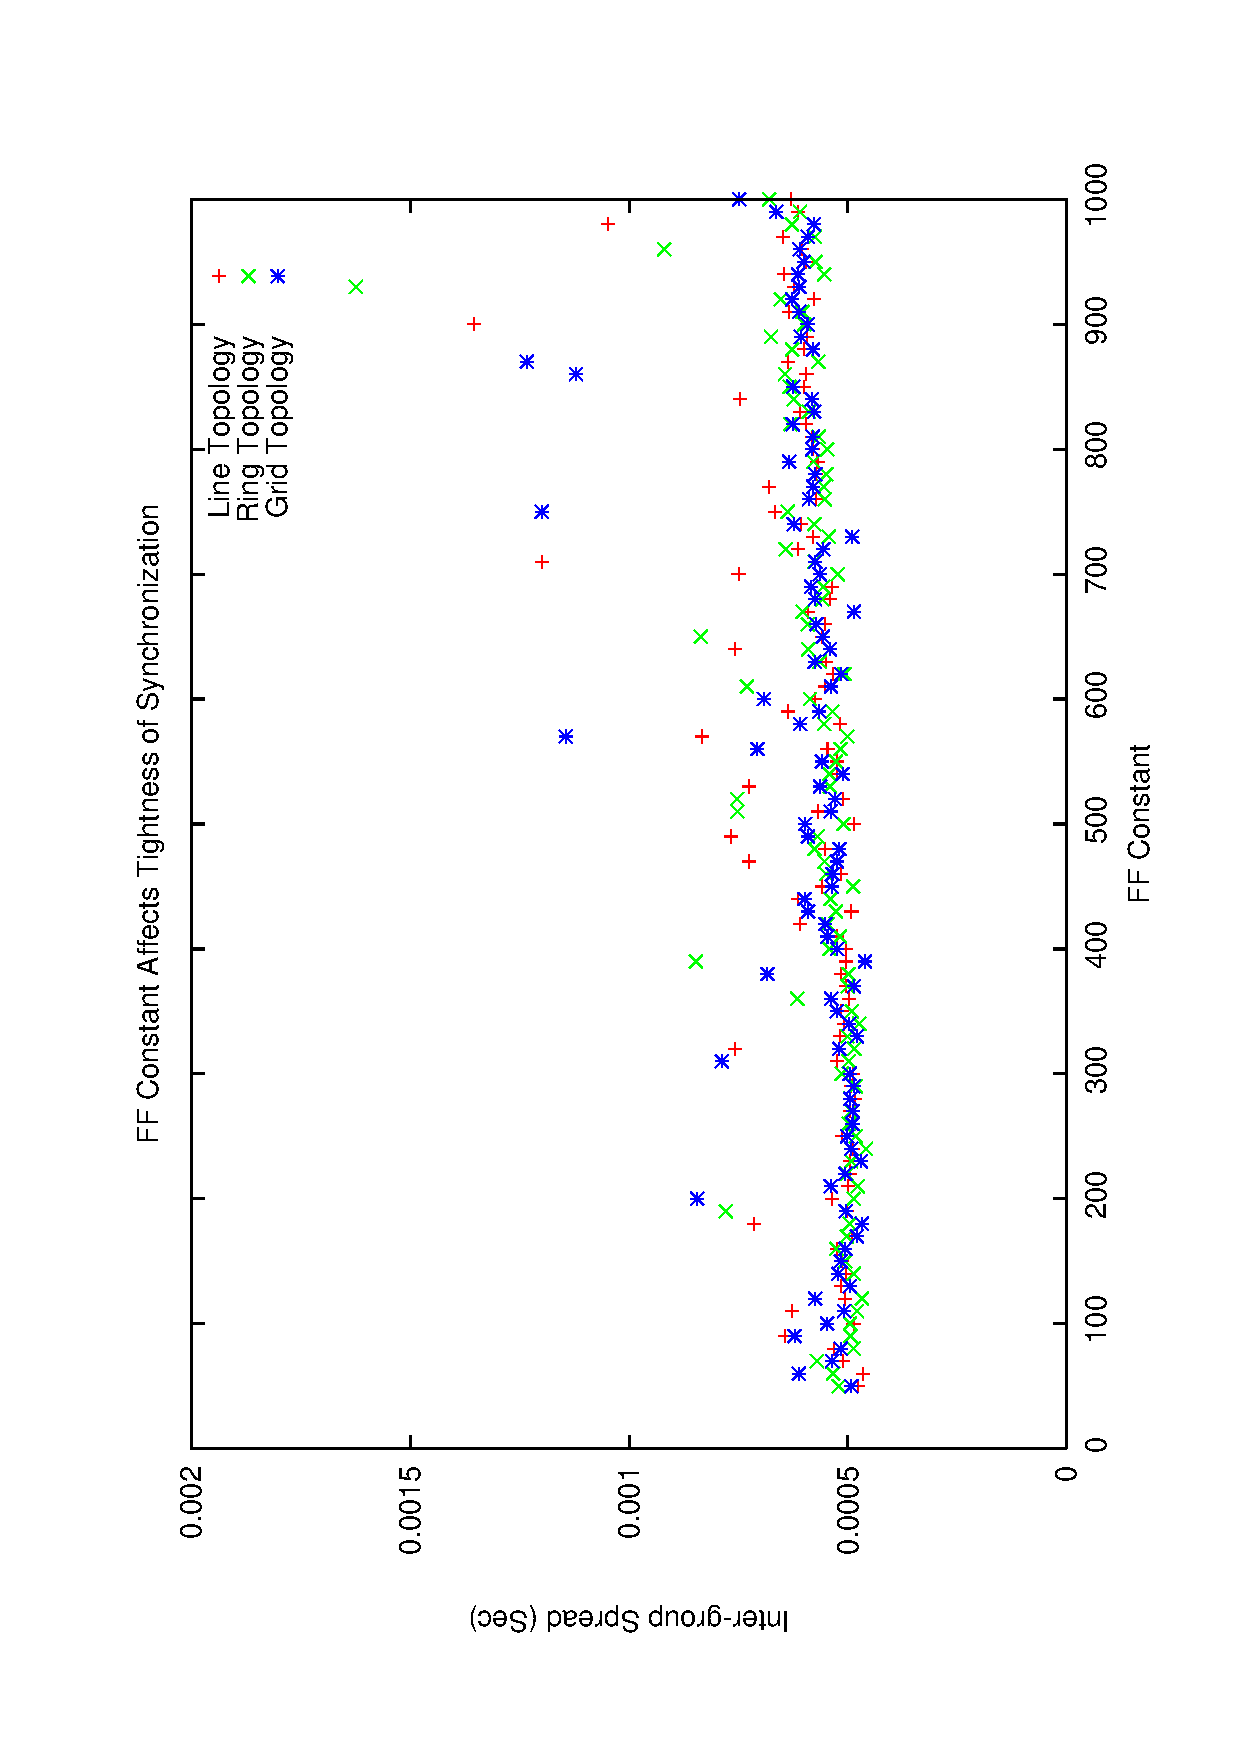
\includegraphics[width=1.0\hsize]{./figures/16-NOADD-LINERINGGRIDALLALL-SPREAD.pdf}
\end{center}
\caption{{\small {\bf The impact of the firing function constant on the group spread for three different node topologies}}}
\label{fig:lgp}
\end{figure}

\begin{figure}[t]
\begin{center}
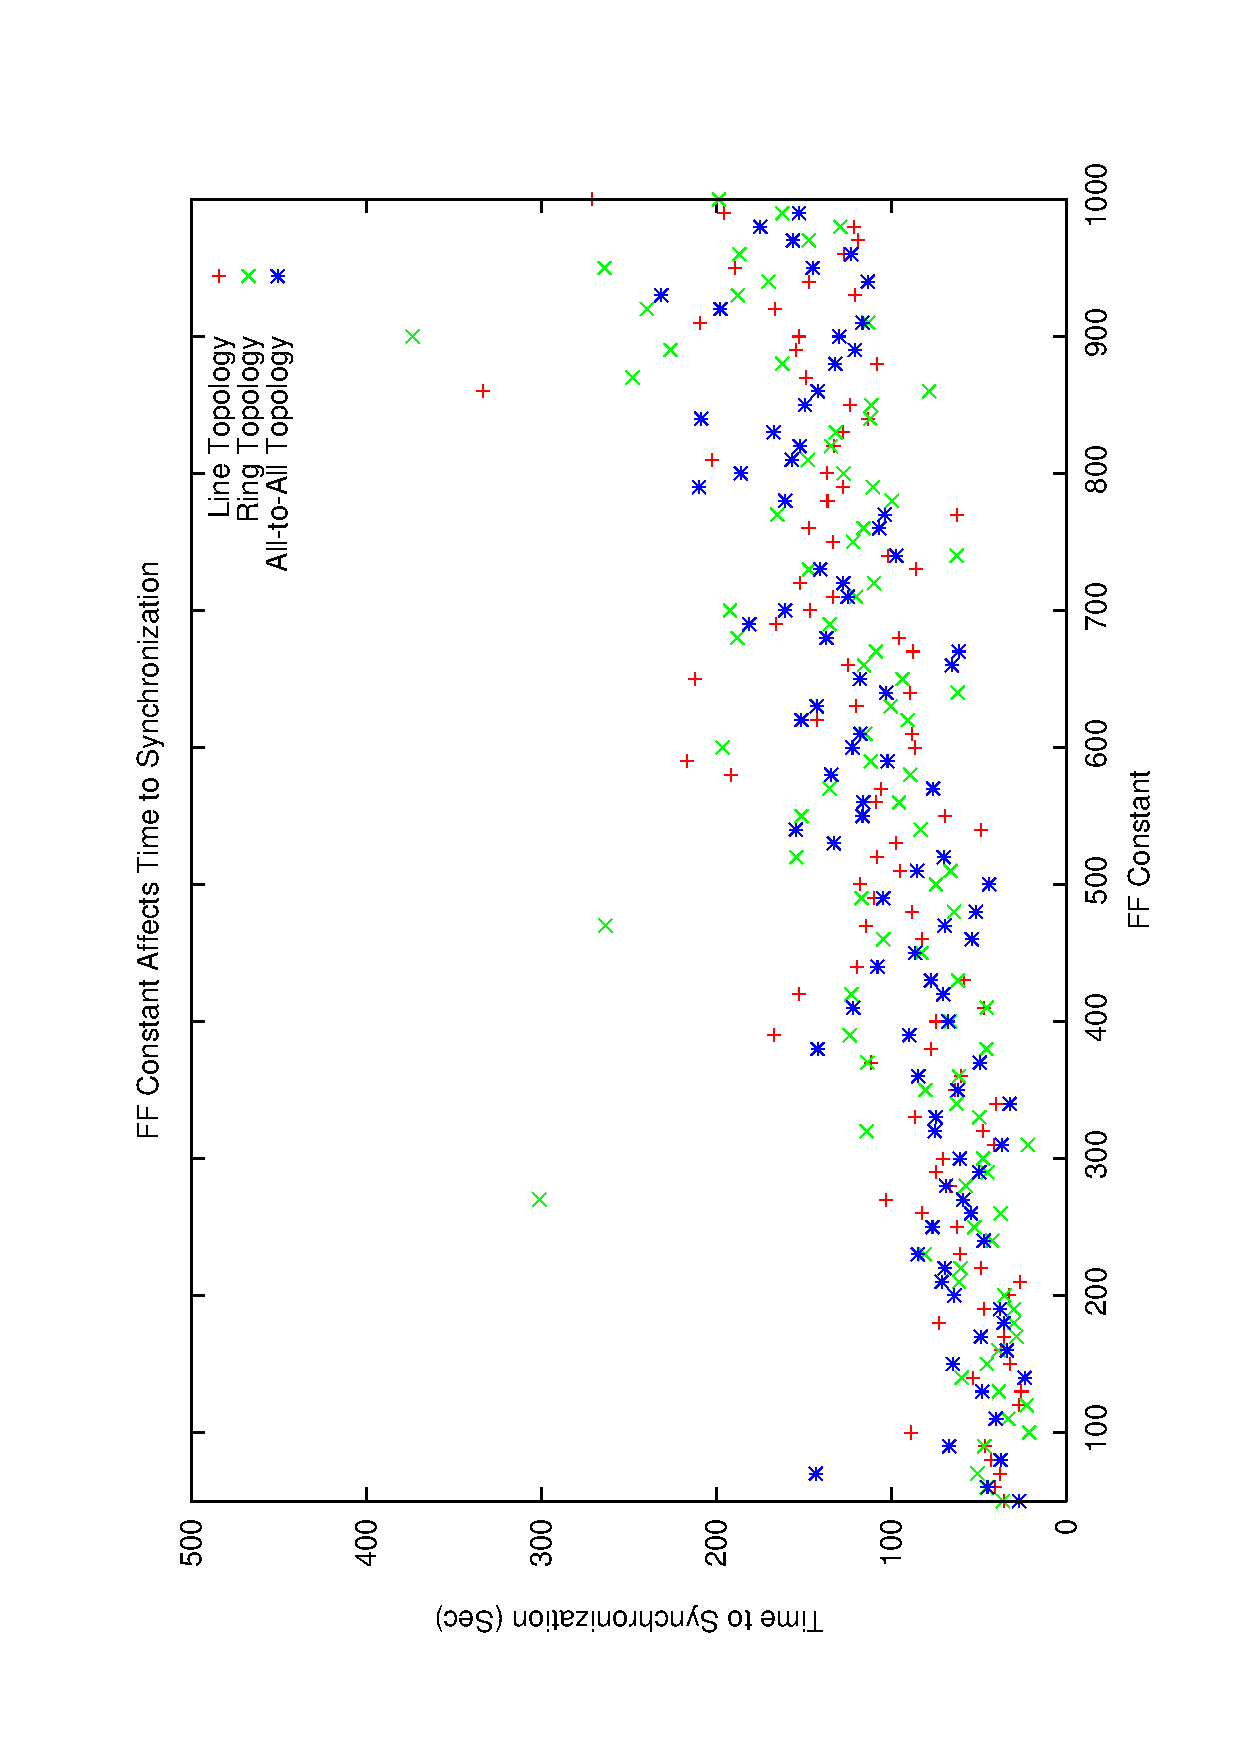
\includegraphics[width=1.0\hsize]{./figures/16-NOADD-LINERINGALLTOALL.pdf}
\end{center}
\caption{{\small {\bf The impact of the firing function constant on the time taken to synchronize for three different node topologies.}}}
\label{fig:lgp}
\end{figure}

\begin{figure}[t]
\begin{center}
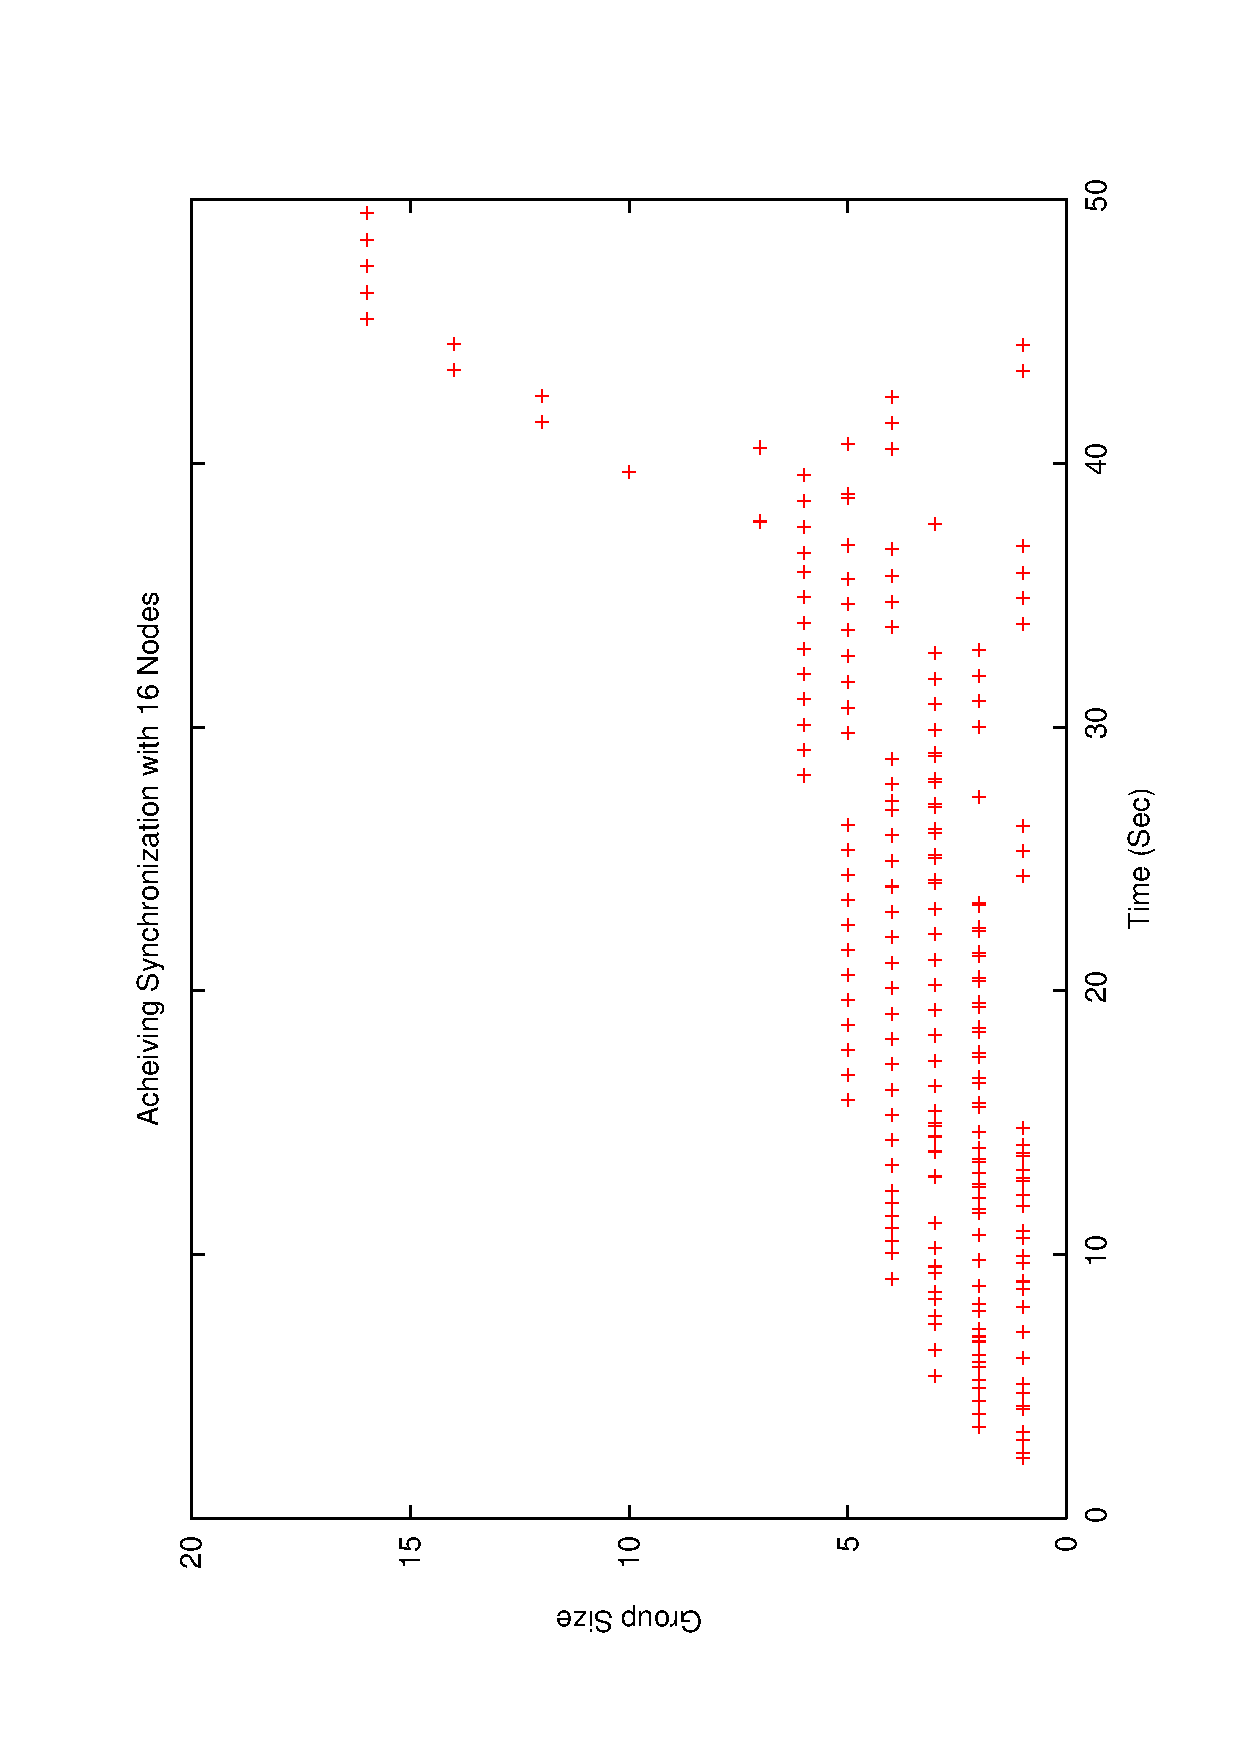
\includegraphics[width=1.0\hsize]{./figures/11-Jan-2005-1-16MOTES-150CONSTANT-RING-EVENT-ALL-GROUPS.pdf}
\end{center}
\caption{{\small {\bf The size of a group over time.}}}
\label{fig:lgp}
\end{figure}